% notes/todo

%TODO - Something about the dispatchers and about what happen when things go right (near-miss)
%TODO - People rarely work alone
%TODO - Something about context and environment
%TODO - Clean up the entire railway section
%TODO - Most standards require an experienced team-member in a given methodogy
%TODO - Organizational structure matters, it is referenced a lot in litterature

%The bureaucracy problem: When people do not sympathize or understand rules and regulation - they tend to bypass them every chance they get. They may even make local modifications to the system to make it fit their need or work flow better.

%Each of them creates a representation of the system using the state of its components, which can be bi-modal (functioning / failure) or multi-modal (several degraded modes and failure modes).

%Variability of performance in humans and organizations comes from their capacity to adapt themselves to working conditions and from the irregularity in activities (perception, cognition, action and communication).


%The second step is determining the potential variability of each operational unit. FRAM classifies operational units into three categories: Human (H), Technical (T) and Organizational (O). The operational unit’s poten tial variability is determined by the respective weights of eleven common performance conditions (CPC), acting as context factors on the operational unit, according to its category. The CPC used in FRAM are based on Hollnagel’s CREAM (Cognitive Reliability and Error Analysis Method) method for studying human reliability; see [9] for a detailed presentation.



%Traditionally, safety systems are modelled as complex linear system, rather than non-linear.

\chapter{Introduction}

\section{Accident investigation}


\section{Terminology}
Safety: freedom from unacceptable risk

%TODO: explain risk matrix

\section{General definitions}

\subsubsection*{Accident}

\subsubsection*{Near miss}
\label{sec:near_miss}
A near miss is often described as "an unplanned event that did not result in injury, illness, or damage - but had the potential to do so". This is also referred to as "Close call" or "Near Collision" when moving objects are involved.\\
\\
Near misses are not, as a rule, taken into consideration as an accident. Whether or not the event should examined and treated as an accident depends largely on how close it was to evolve into a real accident.\\
\\
A recent incident with the Danish IC4 trains resulted in a near miss situation, due to a brake failure. An accident investigation was committed, largely due to the inexplicably of the failure - and the relative young age of the trains.
%A near miss is an unplanned event that did not result in injury, illness, or damage – but had the potential to do so. Only a fortunate break in the chain of events prevented an injury, fatality or damage; in other words, a miss that was nonetheless very near. Although the label of 'human error' is commonly applied to an initiating event, a faulty process or system invariably permits or compounds the harm, and should be the focus of improvement. Other familiar terms for these events is a "close call", or in the case of moving objects, "near collision".

%Find them
A widely spread rule of thumb extrapolates the (Bird, 1974; from Heinrich et Al., 1980) 1:10:30:600 figures giving 1 accident for every 300 near-miss.

A problem with near-misses is they are rarely reported and unsafe acts are considered never reported.

\section{Resonance}

Resonance is a phenomenon in physics making a system oscillate at a higher amplitude when a force is applied. In physics, this is often depicted as a pendulum in motion, where the applied force is the initial push.\\
\\
\cite{hollnagel2004barriers} uses the example of a swing set found on playgrounds. When these are set into motion, one can apply force at just the right time, to increase the amplitude of the oscillating function, that represents the swing. Similarly, you can decrease the amplitude by applying force a bit earlier - hereby damping the kinetic energy of the swing.\\
\\
Resonance can be used to model how large changes in variability can affect and propagate through an entire system. 
%TODO Graph on resonance

\section{Railway}

%Single-track and dual track operation

\subsection{Block}
A block is a distance of railway that, at any point in time can only be occupied by one train. There are two types of blocks; fixed and moving.

Traditionally, railways are divided into a number of fixed blocks with entry and exit signals. These signals will represent train movement along the block based on a predefined policy. The policy is again determined from a number of parameters:


%Ideally, block interlocking policy should be set to match something like

%TODO - change this formula

%$T_{blocking} = 2*WCGF*(WCBT + WCRT)$

%Where

%\begin{itemize}
%  \item $T_{blocking}$ is the amount of time a 
%  \item $WCGF$ is the worst case gradient factor
%  \item $WCBT$ is the worst case braking time
%  \item $WCRT$ is the worst case response time of the driver
%\end{itemize}
Fixed blocks wastes a lot of capacity, as most blocks go largely unused for most of their distance, plus there is a lot of overhead on stopping times.

Moving block address this issue. Instead of having the line divided into a number of fixed blocks, a "safe distance" is defined dynamically based on the current speed and location of the train.
This greatly increases the requirement for the technological infrastructure, and the dependability of it.

Safety has always been a high priority in railway engineering and deployment, and it has thus been a largely contributing industry to safety critical research.

Railway safety is largely dependant on supervision systems, and dispatchers.

\begin{itemize}
  \item The permitted maximum speed on the line
  \item The maximum speed and braking characteristics of the different trains occupying the track
  \item Geological conditions, such as gradients, as these could lead to increase in breaking time.
  \item Line-of-sight. Being that the signal is optical, the train driver must be able to see it before acting on it.
  \item The reaction time of the driver
\end{itemize}
Whereas the maximum speed and geological conditions can be modelled linear - the response time of the driver cannot. And on a line without ATC (see section \ref{sec:atc}) failure to observe a non-go signal will effectively cancel out all other factors in the model.

\subsection{ATC}
\label{sec:atc}
ATC, or Automatic Train Control is a mechanism that allows automatic interlocking of railway blocks.

Barrier in safety engineering

general safety en resilience engineering terminology



\subsection{Level crossing}
%A level crossing (a primarily British term; usually called a "railroad crossing" in the United States) occurs where a railway line is intersected by a road or path on one level, without recourse to a bridge or tunnel. It is a type of at-grade intersection. The term also applies when a light rail line with separate right-of-way or reserved track crosses a road in the same fashion. Other names include railway crossing, grade crossing, road through railroad, or train crossing.

\subsection{Timetable}
The primary barrier to provide safety in railway operation is the timetable. It specifies which trains are supposed at a certain location at a certain point in time. It is considered the first safety measure in railway operation - and thus required all employees to be in possession of a pocket or wrist watch in order for them to be hired.

%\subsection{Dispatcher}
%Maybe deprecate this section
%A train dispatcher can be considered the safety net for when the static timetable needs to altered mid-deployment.
%Dispatchers act on
%\cite{belmonte2008dispatcher}


%\section{Notes}
%Beyond Design-Base Accidents are accidents that occurs as a reaction to unanticipated usage or capacity load. In other words, it's what was no taken into account when the system was designed.

\section{Safety engineering}
Malicious acts, such as sabotage or terrorism, are considered of the scope of safety engineering - but is instead treated by a separate field called security engineering. Natural disasters, such as earthquakes and tsunamis, are also typically left out. These are commonly referred to as "Acts of God" as a unified description.

\section{Barriers}
\label{sec:barriers}
%TODO list the barriers
Depending on the view, domain or application there may be more than one way of categorizing barriers.\cite{hollnagel2004barriers} defines a barrier as:
\begin{quote}
Barriers are hindrances that may either prevent an unwanted event from taking place, or protect against the consequences
\end{quote}
and also defines four categories of barriers; Physical, functional, symbolic and incorporeal.

\begin{itemize}
  \item Physical barrier: A wall, interlock or similar
  \item Functional: 
  \item Symbolic: A sign
  \item Incorporeal: Legislation, procedures
\end{itemize}




\section{Safety Engineering}
Accidents are, in classic safety literature, depicted as a series of sequential events - each one is the causing factor of the next. Stopping the event chain from propagating before it ultimately leads to an injury (or damage), will prevent it. This model is also known as the domino model, due to its close resemblance to a series of dominoes and the way they fall sequential.\\
\\
This reasoning is very easy to follow and makes a lot of sense in simple systems. It is easily depiction and hereby easily communicated. There is also a tendency that people think in linear and sequential systems, rather than in complex intercouplings - as these are far easier to comprehend.\\
\\
But, in general it is not recommended to say that a specific event (X) causes another (Y). This implies that X is a precondition to Y, and by eliminating X, Y will no longer happen\cite{sklet2002methods}.\\
\\
Lundberg et al. also makes a point of this in \cite{lundberg2009you}, as it is titled ``What-You-Look-For-Is-What-You-Find - The consequences of underlying accident models in eight accident investigation manuals''


\subsection{Swiss Cheese Model}

%http://en.wikipedia.org/wiki/Swiss_cheese_model
Barriers are depicted as layers of swiss cheese with holes in them. 


There has been a paradigm shift in the view on accidents in the later years. Now, accidents are not considered a linear succession events, but rather a complex combination of events.


%**Stolen
%Cognitive Reliability and Error Analysis (CREAM) [5]. CREAM allows to highlight the dependence of human performance on the context and provides an useful cognitive model for both retrospective and prospective acci-dent analysis. The specificity of CREAM is that human errors are shaped more bythe context than by a stochastic process.
%/stolen


Current formal requirements on safety measures in systems engineering, usually focus on the robustness and integrity of single components, rather than on the coupling of these and the system as a whole.
\section{Resilience Engineering}
\label{sec:resilience_engineering}
Resilience engineering can be considered the complimentary to safety engineering; where as safety engineering seeks to build a better and safer system, resilience engineering embraces the fact that errors arise within a system - and tries to limit the impact of these.

Whereas traditional risk management rely largely on lessons learned, and empric data to provide probabilities; resilience engineering provocatively seeks to create safety though flexibility. Meaning that when a sub-system breaks down it does not necessarily mean the breakdown of the entire system.

Dynamic reconfiguration is a good example on resilience engineering.
%TODO example

Basically it cuts down to the the following question: "If this component breaks down - how will the rest of the system react, and how can I limit the impact."

%**Stolen
%Resilience Engineering looks for ways to enhance the aility of organisations to create processes that are robust yet flexible, to monitor and revise risk models, and to use resources proactively in the face of disruptions or ongoing production and economic pressures. 
%In Resilience Engineering failures do not stand for a breakdown or malfunctioning of normal system functions, but rather represent the converse of the adaptations necessary to cope with the real world complexity. Individuals and organisations must always adjust their performance to the current conditions; and because resources and time are finite it is inevitable that such adjustments are approximate. Success has been ascribed to the ability of groups, individuals, and organisations to anticipate the changing shape of risk before damage occurs; failure is simply the temporary or permanent absence of that.
%/Stolen

\section{The complexity paradox}
As technology advances, systems become more complex, and as their complexity increased, so does their ability to fail in unpredictable ways. This is mainly caused by the incomprehensible size of the entire system as a whole and the number of components used and their inter-dependency.
A singe component can fail and propagate through the system undetected and be a contributing factor along with others (e.g. environmental or organizational) to the failure of the entire system.\\
\\
As these failure are detected, remedial actions are taken - leading to increasing complexity of the system - effectively amplifying the unpredictability.\\
\\
Computer software is a very good example of a complex system that respond poorly to remedial actions, as resilience is not normally a design goal. A large number of assumptions about values and parameters in a software system can lead to very unpredictable behaviour.\\
\\
Assume the following: a number in a computer system is represented binary form with a fixed size, e.g. 8 places (bits). When representing a negative number the leftmost bit is `1' - or `logic high' which leaves only the remaining 7 bits to represent the actual number. The largest signed number we can represent with 8 bits is $2^8 - 1 = 127$. Due to the nature of computer hardware, the number will "wrap around" - much like in a trip meter in an automobile. The problem with the signed representation is at that for an 8 bit representation, the following holds $(2^8-1)+1 = -128$ which is very inaccurate if you expect a positive value.\\
\\
This is a trivial error, but unfortunately still very common - and will most certainly result in unpredictable behaviour in most systems if not detected.

\chapter{Human factors}
The variability of is system is becoming more and more dependent on individual and/or collective performance of humans, and the need for a model that takes these into account, has arisen.\\
\\
As previously discussed, linear and strongly intercoupled systems are no longer the reality in which we live in anymore. Technological advances has created a self-reinforcing closed loop circuit in which complexity continues to nourish itself (\ref{sec:complexity_loop}).\\
\\
To be able to represent and integrate humans as a part of complex larger system, it is neccesary to idenfity and ultimately accept the behaviours and limits of them.

\section{Human performance}




\subsection{ETTO principle}
The ETTO is short for Effectiveness-Thoroughness-Trade-Off, and the ETTO principle formalizes the balancing issue in having conflicting requirements or goals. The stop-rule (\ref{sec:root_cause_analysis}) is an example of the ETTO principle, as it is usually not possible to do a more in-depth investigation than what time or financial resources allows.\\
\\
ETTO is something most people do every day without giving it much thought. Cooking for instance, may be subject to a time constraint (dinner time), and thus flavouring the food may become under-prioritized in order to meet the deadline. The saying, I've heard in software engineering circles;
 \begin{quote}
 The product will be Fast, Cheap or Good - pick any two
\end{quote}
Seems appropriate here.\\
\\
ETTO is also commonly applied when insufficient information or knowledge is available; sometimes people fail to acknowledge or follow rules simply because they do not comprehend or know the purpose. This is common in layered management systems, where higher layers of management may enforce procedure rules on workers, in order to control, monitor or optimize processes.

\subsection{Feed-forward}
Human behaviour can be regarded as a feed-forward loop, rather than a feed-back loop. In a feed-back loop, you basically respond to the changes and/or information presented to you at the time of their arrival. In feed-forward systems, however, there is a expectation on what will happen next and responses to action are based on the expected effect among a set of responses.\\
\\
A good example is driving a car. Minor corrections are done to the direction of the car, sometimes at a very high frequency of several times a second. This has become second nature to regular drivers, but anyone who has observed another person driving a car would have noticed these minor corrections.\\
The changes done in direction and/or speed of the car are done on the basis on the expectations the driver has to them. In other words, he/she dynamically alters the total system (car+driver) to reflect the desired outcome of the driver - reaching the destination safely.
\subsection{Cognition}
Cognition is popularly referred to as the processes of the mind. It refers to the mental processes that allows memory, abstract problem solving, decision making. The human mind is a complex cognitive system in itself.

The following definition originates from \cite{hollnagel2005joint}.\\
A Cognitive system is
\begin{itemize}
  \item being goal oriented and based on symbol manipulation
  \item being adaptive and able to view a problem in more than one way; and
  \item being able to plan and modify actions based on that knowledge
\end{itemize}
%TODO - finish the section
Cognition is field of study which is best suited for in-field studies and application. This is been widely accepted as "Cognition in the wild".

As people rarely work alone, it makes sense to treat a complete system that involves both humans, organizations and technology as a joint cognitive system. \cite{hollnagel2005joint}\\
\\
Joint cognitives systems are treated by the relative new cognitive systems engineering field, and distance itself from the classic human-machine interface (HMI). It regards the entire system, including the operator, as a whole - rather than two separate isolated systems.
\subsection{Circadian rhythm}
The circadian rhythm is a the natural daily rhythm that is found in, humans, plants, other mammals alike. It has tremendous impact on the performance of an individual and is thus non-negligible when discussing human factors in a system.

Circadian rhythm has a large impact on, for example aeroplane pilots flying across time zones, and thus loses their natural sense of daylight. This leads to fatigue, decreased responsiveness and performance (\cite{mallis2010aircrew}).
%TODO - Add licenseing
\begin{figure}[h]
 \centering
   \includegraphics[width=360pt]{figures/biological_clock_human.pdf}
 \caption{Human biological clock (Licence: GFDL)}
 \label{fig:human_biological_clock}
\end{figure}

\section{User interfaces}
In the recent years, as both cognitive psychology and technical progress has advanced, user interfaces is beginning to receive more attention. 
% The move from analog to digital user interfaces. Digital is just an analog

\cite{norman2002design} presents the human action cycle manifested into the following seven stages of action. The following ordered list presents these steps in specific relation to user interface design - from the users perspective.
\begin{enumerate}

  \item Form a goal: What does the user want to achieve?
  \item Translating the goal into a task or a set of unordered tasks: Which actions are needed to reach the goal?
  \item Order the tasks: 
  \begin{itemize}
     \item Do the users have sufficient domain and task knowledge and sufficient understanding of their work to formulate the action sequence?

     \item Does the UI help the users formulate the action sequence?

  \end{itemize}  
  \item Executing the action sequence:
  \begin{itemize}
     \item Can typical users easily learn and use the UI?
     \item Do the actions provided by the system match those required by the users?
     \item Are the affordance and visibility of the actions good?
     \item Do the users have an accurate mental model of the system?
     \item Does the system support the development of an accurate mental model?
  \end{itemize}  
  \item Perceiving what happened:
  \begin{itemize}
     \item Can the users perceive the system’s state?
     \item Does the UI provide the users with sufficient feedback about the effects of their actions?
  \end{itemize}  
  \item Interpreting the outcome according to the users’ expectations:
  \begin{itemize}
     \item Are the users able to make sense of the feedback?
     \item Does the UI provide enough feedback for this interpretation?
  \end{itemize}  
  \item Evaluating what happened against what was intended
  \begin{itemize}
     \item Can the users compare what happened with what they were hoping to achieve?
  \end{itemize}  

\end{enumerate}


%The door push/pull usability example
Usability engineering is a field in growth

\section{Joint Cognitive Systems}
\cite{hollnagel1983cognitive}
People rarely work alone.
%**Stolen
% The understanding of the human role in accidents has gone through three stages. In the classical view, humans were seen as error prone or as fallible machines. The purpose of an accident investigation was therefore often to find the "human error" that either was the primary (or even "root") cause or the initiating event.
%When it became clear, in the 1990s, that the "human error" view was not tenable, explanations changed to look for how performance shaping factors or performance conditions could make people fail, in the sense of "forcing" errors. This did not remove the concept of a "human error", but saw these as a product of the working conditions and work pressures, rather than as a result of built-in human error tendencies.
%Although this development enabled people to understand accidents of a more complex nature for a while, it still fell short in a number of situations. This led to the recognition, strongly supported by resilience engineering, that failures and successes have the same source, and that they metaphorically speaking are two sides of the same coin.
%The functional resonance model (Hollnagel, 2004) describes system failure as a resonance of the normal variability of functions. To arrive at a description of functional variability and resonance, and to determine recommendations for damping unwanted variability, a FRAM analysis consists of four steps:

%Identify and describe essential system functions, and characterise each function by six basic parameters.
%Characterise the (context dependent) potential variability through common performance conditions.
%Define the functional resonance based on possible dependencies / couplings among functions and the potential for functional variability.
%Identify barriers for variability (damping factors) and specify required performance monitoring.
%/Stolen

\section{Dynamic reconfiguration}
One of the thing human do very differently, and much better, than machines is adapt. Humans are able to learn from experience and apply new knowledge. Machines however, are usually only designed for one purpose, and reconfiguration is usually not an option, unless it is really necessary - e.g. when situation of emergency arises.
%Generel on how dynamic reconfiguration
Modern end-user comsumer products are usually designed with a dynamic reconfiguration strategy in mind - where applicable.

A market where dynamic in-field reconfiguration is widely used, is the growing market for smart phones. These are typically cellular phones with additional functionality, such as being able to install third party software. The makers of these products have acknowledged the fact that their system, due to increasing constraints on time-to-market window, will have to be shipped before extensive testing has been performed.\\
But by enabling their system to be reconfigured in-field, they will be able to fix errors in their product, that have been identified by the users.

\chapter{Accident modelling}

\cite{hollnagel2004barriers} discusses a number of accident models in detail, and finds - among other things - the following:

\begin{itemize}
\item Graphical representation is a big challenge. Both when it comes to communicating the findings, but also when the cause of the accident has to be traced. Boxes and sequential also models tends to lead to boxed and sequential thinking.
\item Complex models are not easily represented graphically, nor are they easy to communicate without loss of information quality, or correctness.
\item Organizational structure is often overlooked and neglected in 
\end{itemize}

Historically, this has not always been so.
%TODO
\section{Moving up the abstraction ladder}
When deploying systems for controlling physical processes, there is a large risk of alienating the people working with the process. Especially if the have not been in touch with the actual process itself, but only with the abstract representation.

A number of unintended constraints will inevitably appear when trying to represent a real system from a model. Especially those of symbols and display screen real estate. Whereas when you are present at the machine itself, you can actually see what is going on.

\cite{hollnagel2005joint}%page 40

\section{Root Cause Analysis}
Sharp and blunt end
%TODO General on RCA
Before starting a RCA, a stop rule is usually defined. A stop rule is the point where you do no dig any further. An analogy from \cite{hollnagel2004barriers} shows a RCA as a tree where the single leaf can be considered an event. The cause is then traced back to the roots of the tree to the root, but usually not any further. A root event can typically be traced further back, and fans out to a number of contributing factors.


\section{Fault tree analysis}
\label{sec:fault_tree_analysis}

\section{FMEA}
%A failure modes and effects analysis (FMEA) is a procedure in product development and operations management for analysis of potential failure modes within a system for classification by the severity and likelihood of the failures. A successful FMEA activity helps a team to identify potential failure modes based on past experience with similar products or processes, enabling the team to design those failures out of the system with the minimum of effort and resource expenditure, thereby reducing development time and costs. It is widely used in manufacturing industries in various phases of the product life cycle and is now increasingly finding use in the service industry. Failure modes are any errors or defects in a process, design, or item, especially those that affect the customer, and can be potential or actual. Effects analysis refers to studying the consequences of those failures.
Failure Mode and Effect Analysis assumes views the system as a number of individual components, and by implying the failure of one of these components, the effect is sought determined. This can be very useful in detecting single-points-of-failure components and perform remedial actions on these. FMEA can also be applied on a functional level, rather than on component level - depending on domain and context.\\
\\
When the failure modes are identified, each is systematically quantified by the following three measurements.

\subsection{Occurrence}
\label{sec:fmea_occurrence}
%In this step it is necessary to look at the cause of a failure mode and the number of times it occurs. This can be done by looking at similar products or processes and the failure modes that have been documented for them in the past. A failure cause is looked upon as a design weakness. All the potential causes for a failure mode should be identified and documented. Again this should be in technical terms. Examples of causes are: erroneous algorithms, excessive voltage or improper operating conditions. A failure mode is given an occurrence ranking (O), again 1–10. Actions need to be determined if the occurrence is high (meaning > 4 for non-safety failure modes and > 1 when the severity-number from step 2 is 9 or 10). This step is called the detailed development section of the FMEA process. Occurrence also can be defined as %. If a non-safety issue happened less than 1%, we can give 1 to it. It is based on your product and customer specification.
The purpose of this step is to determine the frequency of the failure. This is usually usually based around historical or empirical numbers. Each failure mode is given a rating between 1-10 based on the definitions given in table \ref{table:fmea_occurrence}.

\begin{table}[h]
\centering
    \begin{tabular}{ | l | r | }
    \hline
    Rating & Meaning \\ \hline \hline
    1      & No known occurrences on similar products or processes  \\ \hline
    2-3    & Low (relatively few failures) \\ \hline
    4-6    & Moderate (occasional failures) \\ \hline
    7-8    & High (repeated failures) \\ \hline
    9-10   & Very high (failure is almost inevitable) \\ \hline
    \end{tabular}
\caption{FMEA occurrence categories}
\label{table:fmea_occurrence}
\end{table}

\subsection{Severity}
\label{sec:fmea_severity}
%TODO
%Determine all failure modes based on the functional requirements and their effects. Examples of failure modes are: Electrical short-circuiting, corrosion or deformation. A failure mode in one component can lead to a failure mode in another component, therefore each failure mode should be listed in technical terms and for function. Hereafter the ultimate effect of each failure mode needs to be considered. A failure effect is defined as the result of a failure mode on the function of the system as perceived by the user. In this way it is convenient to write these effects down in terms of what the user might see or experience. Examples of failure effects are: degraded performance, noise or even injury to a user. Each effect is given a severity number (S) from 1 (no danger) to 10 (critical). These numbers help an engineer to prioritize the failure modes and their effects. If the sensitivity of an effect has a number 9 or 10, actions are considered to change the design by eliminating the failure mode, if possible, or protecting the user from the effect. A severity rating of 9 or 10 is generally reserved for those effects which would cause injury to a user or otherwise result in litigation.
Next step is to determine the severity of the failure mode - or the effect. If, for example, it is something that cause minor glitches to observant user(s), it will most likely be categorized as "No effect" - or 1.
If on the other hand, it causes injury to the users it is considered hazardous and will be on a 9 or 10.

\begin{table}[h]
\centering
    \begin{tabular}{ | l | r | }
    \hline
    Rating & Meaning \\ \hline \hline
    1      & No effect  \\ \hline
    2      & Very minor \\ \hline
    3      & Minor \\ \hline
    4-6    & Moderate \\ \hline
    7-8    & High \\ \hline
    9-10   & Very high and hazardous \\ \hline
    \end{tabular}
\caption{FMEA severity categories}
\label{table:fmea_severities}
\end{table}


\subsection{Detection}
\label{sec:fmea_detection}
%TODO
%When appropriate actions are determined, it is necessary to test their efficiency. In addition, design verification is needed. The proper inspection methods need to be chosen. First, an engineer should look at the current controls of the system, that prevent failure modes from occurring or which detect the failure before it reaches the customer. Hereafter one should identify testing, analysis, monitoring and other techniques that can be or have been used on similar systems to detect failures. From these controls an engineer can learn how likely it is for a failure to be identified or detected. Each combination from the previous 2 steps receives a detection number (D). This ranks the ability of planned tests and inspections to remove defects or detect failure modes in time. The assigned detection number measures the risk that the failure will escape detection. A high detection number indicates that the chances are high that the failure will escape detection, or in other words, that the chances of detection are low.

%TODO verify these tables
\begin{table}[h]
\centering
    \begin{tabular}{ | l | r | }
    \hline
    Rating & Meaning \\ \hline \hline
    1      & Certain - fault will be caught on test  \\ \hline
    2      & Almost Certain \\ \hline
    3      & High \\ \hline
    4-6    & Moderate \\ \hline
    7-8    & Low \\ \hline
    9-10   & Fault will be passed to customer undetected \\ \hline
    \end{tabular}
\caption{FMEA detectability categories}
\label{table:fmea_detectability}
\end{table}




\subsection{Risk priority number (RPN)}
When the previous three steps are completed, a worksheet is typically produced, which serves as a basis for calculating risk priority numbers - or RPN. It is calculated in with the following formula.

\begin{equation}
RPN = O \cdot S \cdot D
\end{equation}

Where $O$ is the occurrence frequency factor, $S$ is the severity factor and $D$ is the detectability factor.

The activities for FMEA is covered in extensive detail in \cite{MILSTD1629A}.

% Big brother FMCEA
%RPN play an important part in the choice of an action against failure modes. They are threshold values in the evaluation of these actions.

%After ranking the severity, occurrence and detectability the RPN can be easily calculated by multiplying these three numbers: RPN = S × O × D

%This has to be done for the entire process and/or design. Once this is done it is easy to determine the areas of greatest concern. The failure modes that have the highest RPN should be given the highest priority for corrective action. This means it is not always the failure modes with the highest severity numbers that should be treated first. There could be less severe failures, but which occur more often and are less detectable.

%After these values are allocated, recommended actions with targets, responsibility and dates of implementation are noted. These actions can include specific inspection, testing or quality procedures, redesign (such as selection of new components), adding more redundancy and limiting environmental stresses or operating range. Once the actions have been implemented in the design/process, the new RPN should be checked, to confirm the improvements. These tests are often put in graphs, for easy visualization. Whenever a design or a process changes, an FMEA should be updated.

%A few logical but important thoughts come in mind:

%Try to eliminate the failure mode (some failures are more preventable than others)
%Minimize the severity of the failure
%Reduce the occurrence of the failure mode
%Improve the detection

%TODO - maybe small example or disussion

\section{HAZOP}
HAZOP is a short form of HAZard and OPerability study. It uses a set of guide words to create a systematic review of a system. It is originally developed to analyse chemical process systems, but is now used for a variety of systems - including software. The method itself, and the list of guide words are standardized\footnote{BS: IEC61882:2002 Hazard and operability studies (HAZOP studies)}.

%A hazard and operability study (HAZOP) is a structured and systematic examination of a planned or existing process or operation in order to identify and evaluate problems that may represent risks to personnel or equipment, or prevent efficient operation. The HAZOP technique was initially developed to analyze chemical process systems, but has later been extended to other types of systems and also to complex operations and to software systems. A HAZOP is a qualitative technique based on guide-words and is carried out by a multi-disciplinary team (HAZOP team) during a set of meetings.

HAZOP works by first defining components and interfaces - and how they are interconnected. Due to its origin in chemical processing industry, it focuses on the flow between thesis components via the connections. This however, has proven to be a relevant general model for other field - such as computer science. Here the flow is not a material, but information - or a electrical signal.\\
This has added four additional guide words to HAZOP; early, late, before and after.
Upon identification of interconnections of components, a systematic process is started by taking every relevant guide word for each connection and record any findings.


\begin{table}[h]
\centering
    \begin{tabular}{ | l | r | r |}
    \hline
    Guide Word & Meaning                                & Example \\ \hline \hline

    No or Not  & Complete negation of  & No result or reply\\ 
               & the design intent     & when expected \\ \hline
               
    More       & Quantitative increase & Information/material flow rate \\
               &                       & too high \\ \hline

    Less       & Quantitative decrease & Information/material flow rate \\
               &                       & too low  \\ \hline

    As well as & Qualitative           & Extra product/events in\\
               & modification/increase & addition to expected \\ \hline

    Part of    & Qualitative           & Incomplete sequence/activity\\
               & modification/decrease & \\ \hline

    Reverse    & Logical opposite of   &  Reverse flow of traffic,\\
               & the design intent     &  material or current\\ \hline
               
    Other than & Complete substitution &  Other result/outcome than \\ 
               &                       &  expected \\ \hline
    Early      & Relative to the       &  Signal too early in reference\\
               & clock time            &  to system clock\\ \hline

    Late       & Relative to the       &  Signal too early in reference \\
               & clock time            &  to system clock (deadline miss)\\ \hline
               
    Before     & Relating to order     &  Signal arrives earlier in a \\
               & or sequence           &  sequence than intended\\ \hline
               
    After      & Relating to order     &  Signal arrives later in a\\
               & or sequence           &  sequence than intended\\ \hline
    \end{tabular}
\caption{HAZOP guide words}
\label{table:hazop_guide_words}
\end{table}
The data in table \ref{table:hazop_guide_words} is based on the similar table found in \cite{storey1996safety}.

%TODO Small example

\subsection{Discussion}
HAZOP is a strong and formalized method for doing systematic assessment of a complete system. However, it focuses primarily on the couplings between components, and thus fails to capture any propagation there may arise. This can be remedied by the use of fault trees (\ref{sec:fault_tree_analysis})


\section{STAMP}
System-Theoretic Accident Model and Process

\section{Other models}
MORT, SCAT, STEP, MTO, AEB, TRIPOD, change analysis are covered in-depth by \cite{Sklet200429}.


CREAM
\section{Functional Resonance Analytic Model}
%The functional resonance accident model (FRAM; Hollnagel, 2004) describes system failure in terms of the resonance of normal performance variability. This provides a convenient way of representing the non-linear propagation of events and also makes it possible to account for adverse outcomes in cases where there were no manifest malfunctions or failures. The principle of FRAM is to characterise individual system functions independently of how they may be connected in a specific situation. The characterisation of each function ­ or node ­ is done in terms of six aspects and the values of these aspects determine how nodes may be coupled under given conditions. To produce a description of functional variability and potential resonance, and to determine recommendations for damping unwanted variability, a FRAM analysis consists of four steps:


FRAM is designed for systems which both include human and organizational factors. It seeks to avoid the unintended effects of (sequential thinking) other graphical representations. It represents a system as a set of interconnected functions. Each function is represented as a FRAM node - or as the creator informally states; a hexagonal snowflake. An example is shown i figure \ref{fig:fram_node}.


\begin{figure}[h]
 \centering
   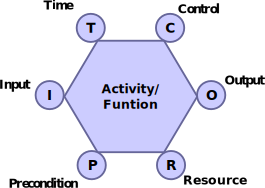
\includegraphics[width=200pt]{figures/FRAM_node.pdf}
 \caption{FRAM node}
 \label{fig:fram_node}
\end{figure}

Each of these nodes consists of a six edge connection points - one output and five inputs. These  model how functions are inter-coupled. A brief explanation of each connector follows.

%Focus on what went right

\begin{itemize}
  %Time available: This can be a constraint but can also be considered as a special kind of resource
  \item Time: Time constraints. Can be real-time or schedule constraints.

%Precondition: System conditions that must be fulfilled before a function can be carried out.
  \item Precondition: A connected function must supply output to this input before the function can start.

% Control: That which supervises or adjusts a function. Can be plans, procedures, guidelines or other functions.
  \item Control: Implies "controlled by", and specifies input from supervising function. Can be plans, procedures, guidelines or other functions.
  
%Input: That which is used or transformed to produce the output. Constitutes Input the link to previous functions.
  \item Input: That which is used or transformed to produce the output. Links to previous functions.

%Output: That which is produced by function. Constitute Output links to subsequent functions.
  \item Output: The basic output of this function - or what it produces. Connects to input of other nodes.
%Resource: That which is needed or consumed by function to process input (e.g.,matter, energy, hardware, software, manpower).
  \item Resource: Resources consumed by this function (examples are; matter, energy, hardware, software, manpower, information)
\end{itemize} 
Unused connectors can explicitly be marked as Not Applicable (N/A).



FRAM analysis basically consists of four steps:

\subsubsection*{Step 1}
%Step 1: Identify essential system functions, and characterise each function by six basic aspects or parameters. The six aspects are input (I, that which the function uses or transforms), output (O, that which the function produces), preconditions (P, conditions that must be fulfilled to perform a function), resources (R, that which the function needs or consumes), time (T, that which affects time availability), and control (C, that which supervises or adjusts the function). Nodes and their aspects may be described in a table and can subsequently visualized in a hexagonal representation (cf. Figure 2 and 4 below).
The objective of the first step is to identify essential system functions, and characterise each of them by the six basic aspects specified in figure \ref{fig:fram_node}. This can be done in a table, and converted to hexagonal objects later on.
%TODO
\subsubsection*{Step 2}
%Step 2: Characterize the context dependent variability of each node. For an accident analysis, the variability is known from the investigation data. In this case the analysis focuses on comparing the observed and the normal performance. For risk assessment, the variability may be derived from a characterisation of the common performance conditions (CPCs), of which there currently are eleven. These CPCs address the combined human, technological, and organizational aspects of each function. After identifying the CPCs, the variability must be determined in a qualitative way in terms of stability, predictability, sufficiency, and boundaries of performance. 
The next step is to characterize the context dependent variability of each node from a list of common performance conditions - or CPCs. 

%The CPC are shown in Table 1, according to operational unit category.
%These context factors can have positive or negative impacts on performance.

%TODO list the eleven CPCs

\begin{table}[h]
\centering
    \begin{tabular}{ | l | r | }
    \hline
    CPC                                                      & Category \\ \hline \hline
    Resource availability                                    &     H-T  \\ \hline
    Training and experience                                  &       H  \\ \hline
    Quality of communications                                &     H-T  \\ \hline
    Quality of human-machine interfaces                      &       T  \\ \hline
    Accessibility and availability of methods and procedures &       H  \\ \hline
    Working conditions                                       &     H-T  \\ \hline
    Number of simultaneous objectives                        &     H-O  \\ \hline
    Time available                                           &       H  \\ \hline
    Circadian rhythm                                         &       H  \\ \hline
    Quality of team collaboration                            &       H  \\ \hline
    Quality of organizational support                        &       O  \\ \hline
    \end{tabular}
\caption{Different CPC's and their category context}
\label{table:cpcs}
\end{table}

After identifying the CPCs, the variability must be determined in a qualitative way in terms of stability, predictability, sufficiency, and boundaries of performance. 

%The quality of each CPC takes one of three possible values: (1) stable or variable but adequate, (2) stable or variable but inadequate, (3) unpredictable. The aim is to determine the set of applicable CPCs for each operational unit and to evaluate their quality.



When applied on an accident analysis, the analysis focuses on comparing the observed and the normal performance.

%**Stolen

\subsubsection*{Step 3}
%Step 3: Defining the functional resonance based on possible dependencies/couplings among functions and the potential for functional variability. The output of the functional description of step 1 is a characterisation of functions and their aspects. The aspects provides the basis for identifying how functions may be coupled. For example, the output of one function may be an input to another function, or produce a resource, fulfil a pre-condition, or enforce a control or time constraint. When the couplings between functions are found, this is combined with the characterization of performance variability from Step 2. In this way the analysis will show how the variability of one function may have an impact on others. This analysis thus determines how resonance, and ultimately adverse outcomes, can result from variability across functions in the system. For example, if the output of a function is unpredictably variable, another function that depends on this output as a resource may be performed unpredictably. Many such occurrences and propagations of variability may have an effect like resonance.
The third step will link the functions and define the functional resonance. The purpose of the couplings between the nodes is to determine the potential for functional variability.


%Step 4: Identify barriers for variability (damping factors) and specify required performance monitoring. Barriers are hindrances that may either prevent an unwanted event from taking place, or protect against the consequences (Hollnagel, 2004). Barriers can be described in terms of barrier systems (the organizational and/or physical structure of the barrier) and barrier functions (the manner by which the barrier achieves its purpose). In FRAM, four categories of barrier systems are identified (each with their potential barrier functions, see Hollnagel, 2004). In addition to recommendations for barriers, FRAM can also be used to specify recommendations for the monitoring of performance and variability, as a way to detect and manage undesired variability. Performance indicators may thus be developed for every function and every link between functions.
\subsection*{Sted 4}
The final step will be be the remedial one, where identification of variability barriers - or damping factors - will take place. For a more in-depth description on barriers see section \ref{sec:barriers}.\\
\\
Usually one or more of these four classes of barriers are deployed;
\begin{itemize}
  \item Monitoring: a management layer barrier that can provide early warning signals to higher levels of management. Usually implemented with the data already available.
  \item Detection: is the technological approach to monitoring, but still requires a manual reasoning and/or interpretation.
  \item Dispersion: involves creating a new physical barrier that prevents propagation - e.g. sprinkler system and airbags. Measures done here are meant to increase the internal resilience of the system.
  \item Correction: can be everything from revised legislations to replacing technological components. It can also involve firing an employee identified as a contributing or causing factor.
\end{itemize}

\section{Retrospective FRAM}
Although FRAM is intended to be used as a pre-deployment tool to enhance the resilience of a system (or sub-system), its modelling characteristics enables it to be applied retrospective on an accident or near-miss event.\\
\\

%**Stolen
%How to use FRAM for event analysis (retrospective)
%An analysis using FRAM comprises the following five steps:
%Define the purpose of modelling and describe the situation being analysed. Either an event that has occurred (incident/accident) or a possible future scenario (risk).
%Identify the essential functions that make up the event ('foreground' functions – when things go right); characterise each by six basic aspects (Input, Output, Pre-conditions, Resources, Time, and Control). 
%Characterise the actual / potential variability of 'foreground' functions and 'background' functions (context). Consider both normal and worst case variability.
%Define functional resonance based on potential  / actual dependencies (couplings) among functions.
%Propose ways to monitor and dampen performance variability (indicators, barriers, design / modification, etc.)
%/Stolen

\section{FRAM tools}
A special-purpose piece of computer software exists to visualize the FRAM models and conveniently describe the functions and couplings using textual input and graphical representation.


\subsection{Fram Visualizer}


\begin{figure}
 \centering
   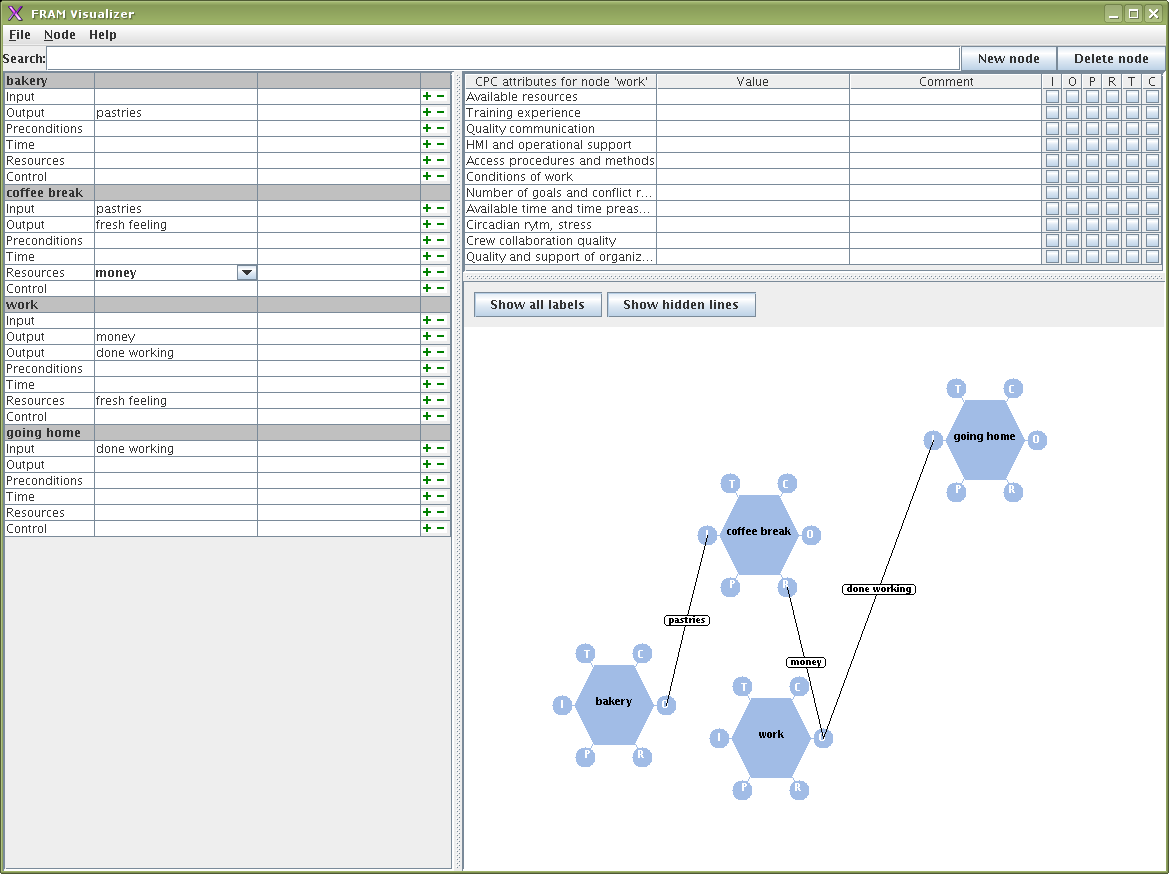
\includegraphics[width=320pt]{figures/framvisualizer1.png}
 \caption{FRAM Visualizer interface}
 \label{fig:fram_visualizer_interface}
\end{figure}


